\section{Minimal Working Example}

\section{Overview}

This section provides a concrete instantiation of the RCO protocol in a minimal configuration sufficient to demonstrate its correctness, implementability, and end-to-end execution. The objective is to construct the smallest system that satisfies all protocol invariants while remaining simple enough for direct implementation and verification.

The minimal system consists of:
\begin{equation}
\mathcal{N} = \{\text{Producer}, V_1, V_2, V_3, \text{Verifier}\}
\end{equation}

with a threshold:
\begin{equation}
t = 2
\end{equation}

such that at least two validators are required to produce a valid proof.

\section{System Initialization}

\subsection{Key Generation}

A distributed key generation process produces:

\begin{equation}
(K_1, K_2, K_3), \quad PK
\end{equation}

where each $K_i$ is a private key share and $PK$ is the public key.

\subsection{Initial State}

The system initializes:

\begin{equation}
L_0 = \mathcal{H}(0)
\end{equation}

\begin{equation}
S_0 = \text{initial system state}
\end{equation}

\section{Telemetry Instance}

Consider a concrete telemetry input:

\begin{equation}
D_1 = \{\text{temperature}: 25.0, \text{pressure}: 1.01\}
\end{equation}

\subsection{Canonical Serialization}

Applying $\mathcal{S}$:

\begin{equation}
B_1 = \texttt{"pressure:1.01|temperature:25.0"}
\end{equation}

\section{Hash Computation}

\begin{equation}
H_1 = \mathcal{H}(B_1)
\end{equation}

\section{Lineage Update}

\begin{equation}
L_1 = \mathcal{H}(H_1 \concat L_0)
\end{equation}

\section{State Binding}

Assume:

\begin{equation}
S_1 = \text{system state after processing } D_1
\end{equation}

Compute:

\begin{equation}
M_1 = \mathcal{H}_S(S_1) \concat L_1
\end{equation}

\section{Validator Signing}

Each validator computes:

\begin{equation}
\sigma_i = \text{Sign}_i(M_1, K_i)
\end{equation}

Select two validators:

\begin{equation}
\Sigma_1 = \text{Aggregate}(\sigma_1, \sigma_2)
\end{equation}

\section{Verification}

The verifier computes:

\begin{equation}
\text{Verify}(M_1, \Sigma_1, PK) = \text{true}
\end{equation}

Thus:

\begin{equation}
\mathcal{I}_{\text{RCO}}(D_1, L_0) = \text{accept}
\end{equation}

\section{End-to-End Consistency}

The final record is:

\begin{equation}
\mathcal{R}_1 = (D_1, B_1, H_1, L_1, \Sigma_1)
\end{equation}

which satisfies all protocol invariants.

\section{Minimal Correctness Property}

\begin{equation}
\text{accept}(D_1) \implies \text{Valid}(D_1)
\end{equation}

demonstrating correctness of the minimal system.

\section{Conclusion}

This minimal working example demonstrates that the RCO protocol can be instantiated with a small number of components while preserving its full integrity guarantees. The example provides a concrete foundation for implementation and validates the practical feasibility of the protocol.

\section{Pseudocode and Execution Trace}

This section provides a detailed pseudocode specification of the RCO protocol along with a step-by-step execution trace across multiple telemetry events. The objective is to demonstrate that the protocol can be directly implemented in a computational system while preserving its formal guarantees.

\section{Core Pseudocode Definitions}

\subsection{Canonical Serialization Function}

\begin{verbatim}
function CANONICALIZE(D):
    keys = SORT_KEYS(D)
    buffer = ""
    for k in keys:
        buffer += k + ":" + TO_STRING(D[k]) + "|"
    return buffer.strip("|")
\end{verbatim}

\subsection{Hash Function Wrapper}

\begin{verbatim}
function HASH(data):
    return SHA256(data)
\end{verbatim}

\subsection{Lineage Update Function}

\begin{verbatim}
function UPDATE_LINEAGE(H_t, L_prev):
    return HASH(H_t + L_prev)
\end{verbatim}

\subsection{State Binding Function}

\begin{verbatim}
function BIND_STATE(S_t, L_t):
    return HASH(SERIALIZE_STATE(S_t)) + L_t
\end{verbatim}

\subsection{Validator Signing}

\begin{verbatim}
function SIGN_PARTIAL(M_t, K_i):
    return SIGN(M_t, K_i)
\end{verbatim}

\subsection{Aggregation Function}

\begin{verbatim}
function AGGREGATE(signatures):
    return COMBINE(signatures)
\end{verbatim}

\subsection{Verification Function}

\begin{verbatim}
function VERIFY(M_t, Sigma_t, PK):
    return VERIFY_SIGNATURE(M_t, Sigma_t, PK)
\end{verbatim}

\subsection{Full Ingestion Pipeline}

\begin{verbatim}
function INGEST(D_t, S_t, L_prev, validators, threshold):
    B_t = CANONICALIZE(D_t)
    H_t = HASH(B_t)
    L_t = UPDATE_LINEAGE(H_t, L_prev)
    M_t = BIND_STATE(S_t, L_t)

    partial_sigs = []
    for V in validators:
        if V.verify_locally(D_t, S_t, L_prev):
            partial_sigs.append(SIGN_PARTIAL(M_t, V.K_i))

    if len(partial_sigs) < threshold:
        return REJECT

    Sigma_t = AGGREGATE(partial_sigs)

    if VERIFY(M_t, Sigma_t, PK):
        return (ACCEPT, L_t, Sigma_t)
    else:
        return REJECT
\end{verbatim}

\section{Step-by-Step Execution Trace}

We now demonstrate execution over multiple time steps.

\subsection{Initial Conditions}

\begin{equation}
L_0 = \mathcal{H}(0)
\end{equation}

\subsection{Step 1: First Telemetry Input}

\begin{equation}
D_1 = \{\text{temperature}: 25.0, \text{pressure}: 1.01\}
\end{equation}

\paragraph{Canonicalization}

\begin{equation}
B_1 = \texttt{"pressure:1.01|temperature:25.0"}
\end{equation}

\paragraph{Hashing}

\begin{equation}
H_1 = \mathcal{H}(B_1)
\end{equation}

\paragraph{Lineage}

\begin{equation}
L_1 = \mathcal{H}(H_1 \concat L_0)
\end{equation}

\paragraph{State Binding}

\begin{equation}
M_1 = \mathcal{H}_S(S_1) \concat L_1
\end{equation}

\paragraph{Signing and Aggregation}

\begin{equation}
\Sigma_1 = \text{Aggregate}(\sigma_1, \sigma_2)
\end{equation}

\paragraph{Verification}

\begin{equation}
\text{Verify}(M_1, \Sigma_1, PK) = \text{true}
\end{equation}

\subsection{Step 2: Second Telemetry Input}

\begin{equation}
D_2 = \{\text{temperature}: 26.0, \text{pressure}: 1.02\}
\end{equation}

\paragraph{Canonicalization}

\begin{equation}
B_2 = \texttt{"pressure:1.02|temperature:26.0"}
\end{equation}

\paragraph{Hashing}

\begin{equation}
H_2 = \mathcal{H}(B_2)
\end{equation}

\paragraph{Lineage}

\begin{equation}
L_2 = \mathcal{H}(H_2 \concat L_1)
\end{equation}

\paragraph{State Binding}

\begin{equation}
M_2 = \mathcal{H}_S(S_2) \concat L_2
\end{equation}

\paragraph{Signing}

\begin{equation}
\sigma_i^{(2)} = \text{Sign}_i(M_2, K_i)
\end{equation}

\paragraph{Aggregation}

\begin{equation}
\Sigma_2 = \text{Aggregate}(\sigma_1^{(2)}, \sigma_3^{(2)})
\end{equation}

\paragraph{Verification}

\begin{equation}
\text{Verify}(M_2, \Sigma_2, PK) = \text{true}
\end{equation}

\subsection{State Evolution}

The lineage evolves as:

\begin{equation}
L_0 \rightarrow L_1 \rightarrow L_2
\end{equation}

Each step satisfies:

\begin{equation}
L_t = \mathcal{H}(H_t \concat L_{t-1})
\end{equation}

\subsection{Determinism Property}

For any node $i$:

\begin{equation}
L_t^{(i)} = L_t
\end{equation}

ensuring consistency.

\section{Failure Case Demonstration}

Consider an adversarial modification:

\begin{equation}
D_2' = \{\text{temperature}: 30.0, \text{pressure}: 1.02\}
\end{equation}

Then:

\begin{equation}
B_2' \neq B_2 \implies H_2' \neq H_2 \implies L_2' \neq L_2
\end{equation}

Thus:

\begin{equation}
\text{Verify}(M_2', \Sigma_2, PK) = \text{false}
\end{equation}

and the input is rejected.

\section{Execution Invariant}

For all steps:

\begin{equation}
\text{accept}(D_t) \implies
\begin{cases}
\text{deterministic encoding} \\
\text{valid lineage} \\
\text{state consistency} \\
\text{verified proof}
\end{cases}
\end{equation}

\section{Conclusion}

The pseudocode and execution trace demonstrate that the RCO protocol can be implemented using standard computational primitives while preserving its formal guarantees. The step-by-step execution confirms that the system maintains deterministic behavior, rejects invalid inputs, and ensures consistent state evolution across all nodes.

\section{Reference Implementation, System Constraints, and Deployment Mapping}

This section provides a concrete reference implementation outline of the RCO protocol, defines system-level constraints required for correct operation, and maps the protocol to real-world software and infrastructure stacks. The objective is to demonstrate that the protocol can be deployed using existing technologies while preserving its formal guarantees.

\section{Reference Implementation Architecture}

A minimal reference implementation consists of the following modules:

\begin{equation}
\mathcal{M} = \{\text{Ingestion Service}, \text{Validator Nodes}, \text{Aggregation Service}, \text{Storage Engine}, \text{Verification Service}\}
\end{equation}

Each module corresponds directly to components defined in the architectural model.

\subsection{Ingestion Service}

The ingestion service implements the deterministic pipeline:

\begin{verbatim}
INPUT: D_t, S_t, L_prev
OUTPUT: L_t, Sigma_t, status

1. B_t = CANONICALIZE(D_t)
2. H_t = HASH(B_t)
3. L_t = HASH(H_t + L_prev)
4. M_t = HASH_STATE(S_t) + L_t
5. DISPATCH M_t to validators
\end{verbatim}

\subsection{Validator Node}

Each validator node executes:

\begin{verbatim}
INPUT: M_t
OUTPUT: sigma_i

1. if LOCAL_VERIFY(M_t):
2.     sigma_i = SIGN(M_t, K_i)
3.     return sigma_i
4. else:
5.     return null
\end{verbatim}

\subsection{Aggregation Service}

\begin{verbatim}
INPUT: {sigma_i}
OUTPUT: Sigma_t

1. if count(valid signatures) >= threshold:
2.     Sigma_t = AGGREGATE(signatures)
3.     return Sigma_t
4. else:
5.     return REJECT
\end{verbatim}

\subsection{Verification Service}

\begin{verbatim}
INPUT: M_t, Sigma_t
OUTPUT: decision

1. if VERIFY(M_t, Sigma_t, PK):
2.     return ACCEPT
3. else:
4.     return REJECT
\end{verbatim}

\subsection{Storage Engine}

The storage engine maintains:

\begin{verbatim}
append_only_log = []

function STORE(record):
    append_only_log.append(record)
\end{verbatim}

\section{System Constraints}

The correct operation of the RCO protocol requires the following constraints.

\subsection{Deterministic Serialization Constraint}

\begin{equation}
\forall D, \quad \mathcal{S}(D) \text{ must be canonical}
\end{equation}

Any violation leads to divergence across nodes.

\subsection{Cryptographic Assumptions}

The system relies on:

\begin{equation}
\mathcal{H}, \mathcal{H}_S \text{ are collision-resistant}
\end{equation}

\begin{equation}
\text{Signature scheme is EUF-CMA secure}
\end{equation}

\subsection{Threshold Constraint}

\begin{equation}
f < t \leq n
\end{equation}

where $f$ is the number of faulty validators.

\subsection{Network Constraint}

The system assumes eventual message delivery:

\begin{equation}
\forall m, \quad \text{delivered}(m) \text{ within finite time}
\end{equation}

\subsection{State Consistency Constraint}

All nodes must compute:

\begin{equation}
S_t^{(i)} = S_t^{(j)}
\end{equation}

for identical inputs.

\section{Minimal Deployment Diagram}

The system may be deployed as:

\begin{equation}
\text{Producer} \rightarrow \text{Ingestion Service} \rightarrow \text{Validator Cluster} \rightarrow \text{Aggregator} \rightarrow \text{Verifier} \rightarrow \text{Storage}
\end{equation}

\subsection{Logical Flow}

\begin{enumerate}
\item Producer emits telemetry
\item Ingestion service processes and forwards message
\item Validators independently sign
\item Aggregator combines signatures
\item Verifier confirms validity
\item Storage persists record
\end{enumerate}

\subsection{TikZ Deployment Template}

\begin{verbatim}
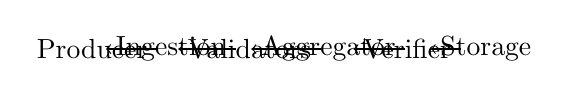
\begin{tikzpicture}
\node (prod) {Producer};
\node (ingest) [right of=prod] {Ingestion};
\node (validators) [right of=ingest] {Validators};
\node (agg) [right of=validators] {Aggregator};
\node (verify) [right of=agg] {Verifier};
\node (store) [right of=verify] {Storage};

\draw[->] (prod) -- (ingest);
\draw[->] (ingest) -- (validators);
\draw[->] (validators) -- (agg);
\draw[->] (agg) -- (verify);
\draw[->] (verify) -- (store);
\end{tikzpicture}
\end{verbatim}

\section{Real-World Technology Mapping}

The RCO protocol can be implemented using existing technologies as follows.

\subsection{Programming Languages}

\begin{itemize}
\item Go: for concurrency and networking
\item Rust: for memory safety and cryptographic operations
\item Python: for prototyping and orchestration
\end{itemize}

\subsection{Cryptographic Libraries}

\begin{itemize}
\item OpenSSL or libsodium for hashing and signatures
\item BLS signature libraries for aggregation
\end{itemize}

\subsection{Networking Layer}

\begin{itemize}
\item gRPC for inter-node communication
\item REST APIs for external interaction
\end{itemize}

\subsection{Storage Systems}

\begin{itemize}
\item Append-only logs using Kafka or Pulsar
\item Persistent storage using PostgreSQL or distributed databases
\end{itemize}

\subsection{Deployment Infrastructure}

\begin{itemize}
\item Containerization using Docker
\item Orchestration using Kubernetes
\item Cloud deployment on distributed regions
\end{itemize}

\section{Scalability and Deployment Constraints}

\subsection{Horizontal Scaling}

\begin{equation}
\text{Throughput} \propto |\mathcal{V}|
\end{equation}

\subsection{Latency Bound}

\begin{equation}
T_{\text{latency}} = \max(T_{\text{sign}}) + T_{\text{network}} + T_{\text{agg}}
\end{equation}

\subsection{Fault Isolation}

\begin{equation}
\text{Failure}(V_i) \not\implies \text{Failure}(V_j)
\end{equation}

\section{End-to-End Deployment Invariant}

\begin{equation}
\forall t, \quad \text{Stored}(R_t) \implies \text{Valid}(D_t)
\end{equation}

\section{Implementation Feasibility Statement}

The RCO protocol requires only standard computational primitives:

\begin{equation}
\{\text{hashing}, \text{signatures}, \text{networking}, \text{storage}\}
\end{equation}

and does not depend on specialized hardware or non-standard assumptions.

\section{Conclusion}

This section demonstrates that the RCO protocol can be implemented using existing technologies and deployed in real-world environments. The reference implementation, system constraints, and deployment mapping collectively establish the practical feasibility of the protocol, confirming that its formal guarantees can be realized in operational systems. This completes the minimal working example and validates the end-to-end applicability of the RCO framework.